\documentclass{beamer}

\mode<presentation>
{
  \usetheme{default}      % or try Darmstadt, Madrid, Warsaw, ...
  \usecolortheme{default} % or try albatross, beaver, crane, ...
  \usefonttheme{default}  % or try serif, structurebold, ...
  \setbeamertemplate{navigation symbols}{}
  \setbeamertemplate{caption}[numbered]
}

\usepackage[english]{babel}
\usepackage[utf8x]{inputenc}

\title[RoFi]{RoFi}
\author{Jan Mrázek, Viktória Vozárová}
\institute{Paradise}
\date{21. 5. 2018}

\begin{document}

\begin{frame}
  \titlepage
\end{frame}

\section{Úvod}

\begin{frame}{Co je naším cílem?}

    Vyvinout rekonfigurovatelnou distribuovanou robotickou platformu.

    \begin{center}
    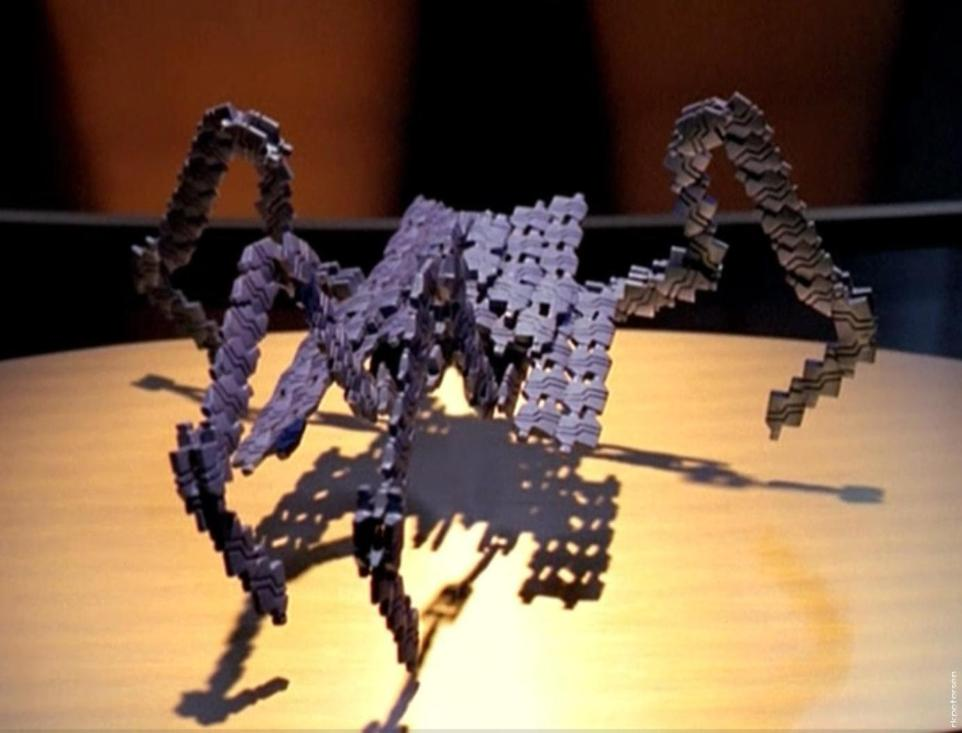
\includegraphics[width=0.7\textwidth]{img/replicator2}

    ...v podstatě Replikátory z StarGate SG-1.

    \url{https://youtu.be/gm0KUVByx40?t=49}
    \end{center}

\end{frame}

\begin{frame}{Co je to replikátor?}
    \begin{center}
        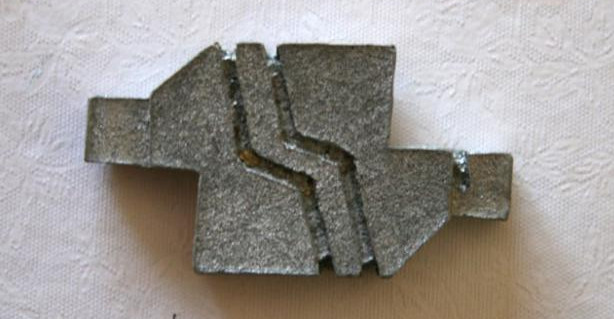
\includegraphics[width=0.6\textwidth]{img/replicator3}
    \end{center}

    \begin{columns}
        \begin{column}{0.5\textwidth}
            \begin{itemize}
                \item robot
                \item rekonfigurovatelný
                \item distribuovaný
            \end{itemize}
        \end{column}
        \begin{column}{0.5\textwidth}
            \begin{itemize}
                \item využívá prostředí
                \item nepřátelský
                \item snaží se ovládnout svět
            \end{itemize}
        \end{column}
    \end{columns}
\end{frame}

\begin{frame}{RoFi}
    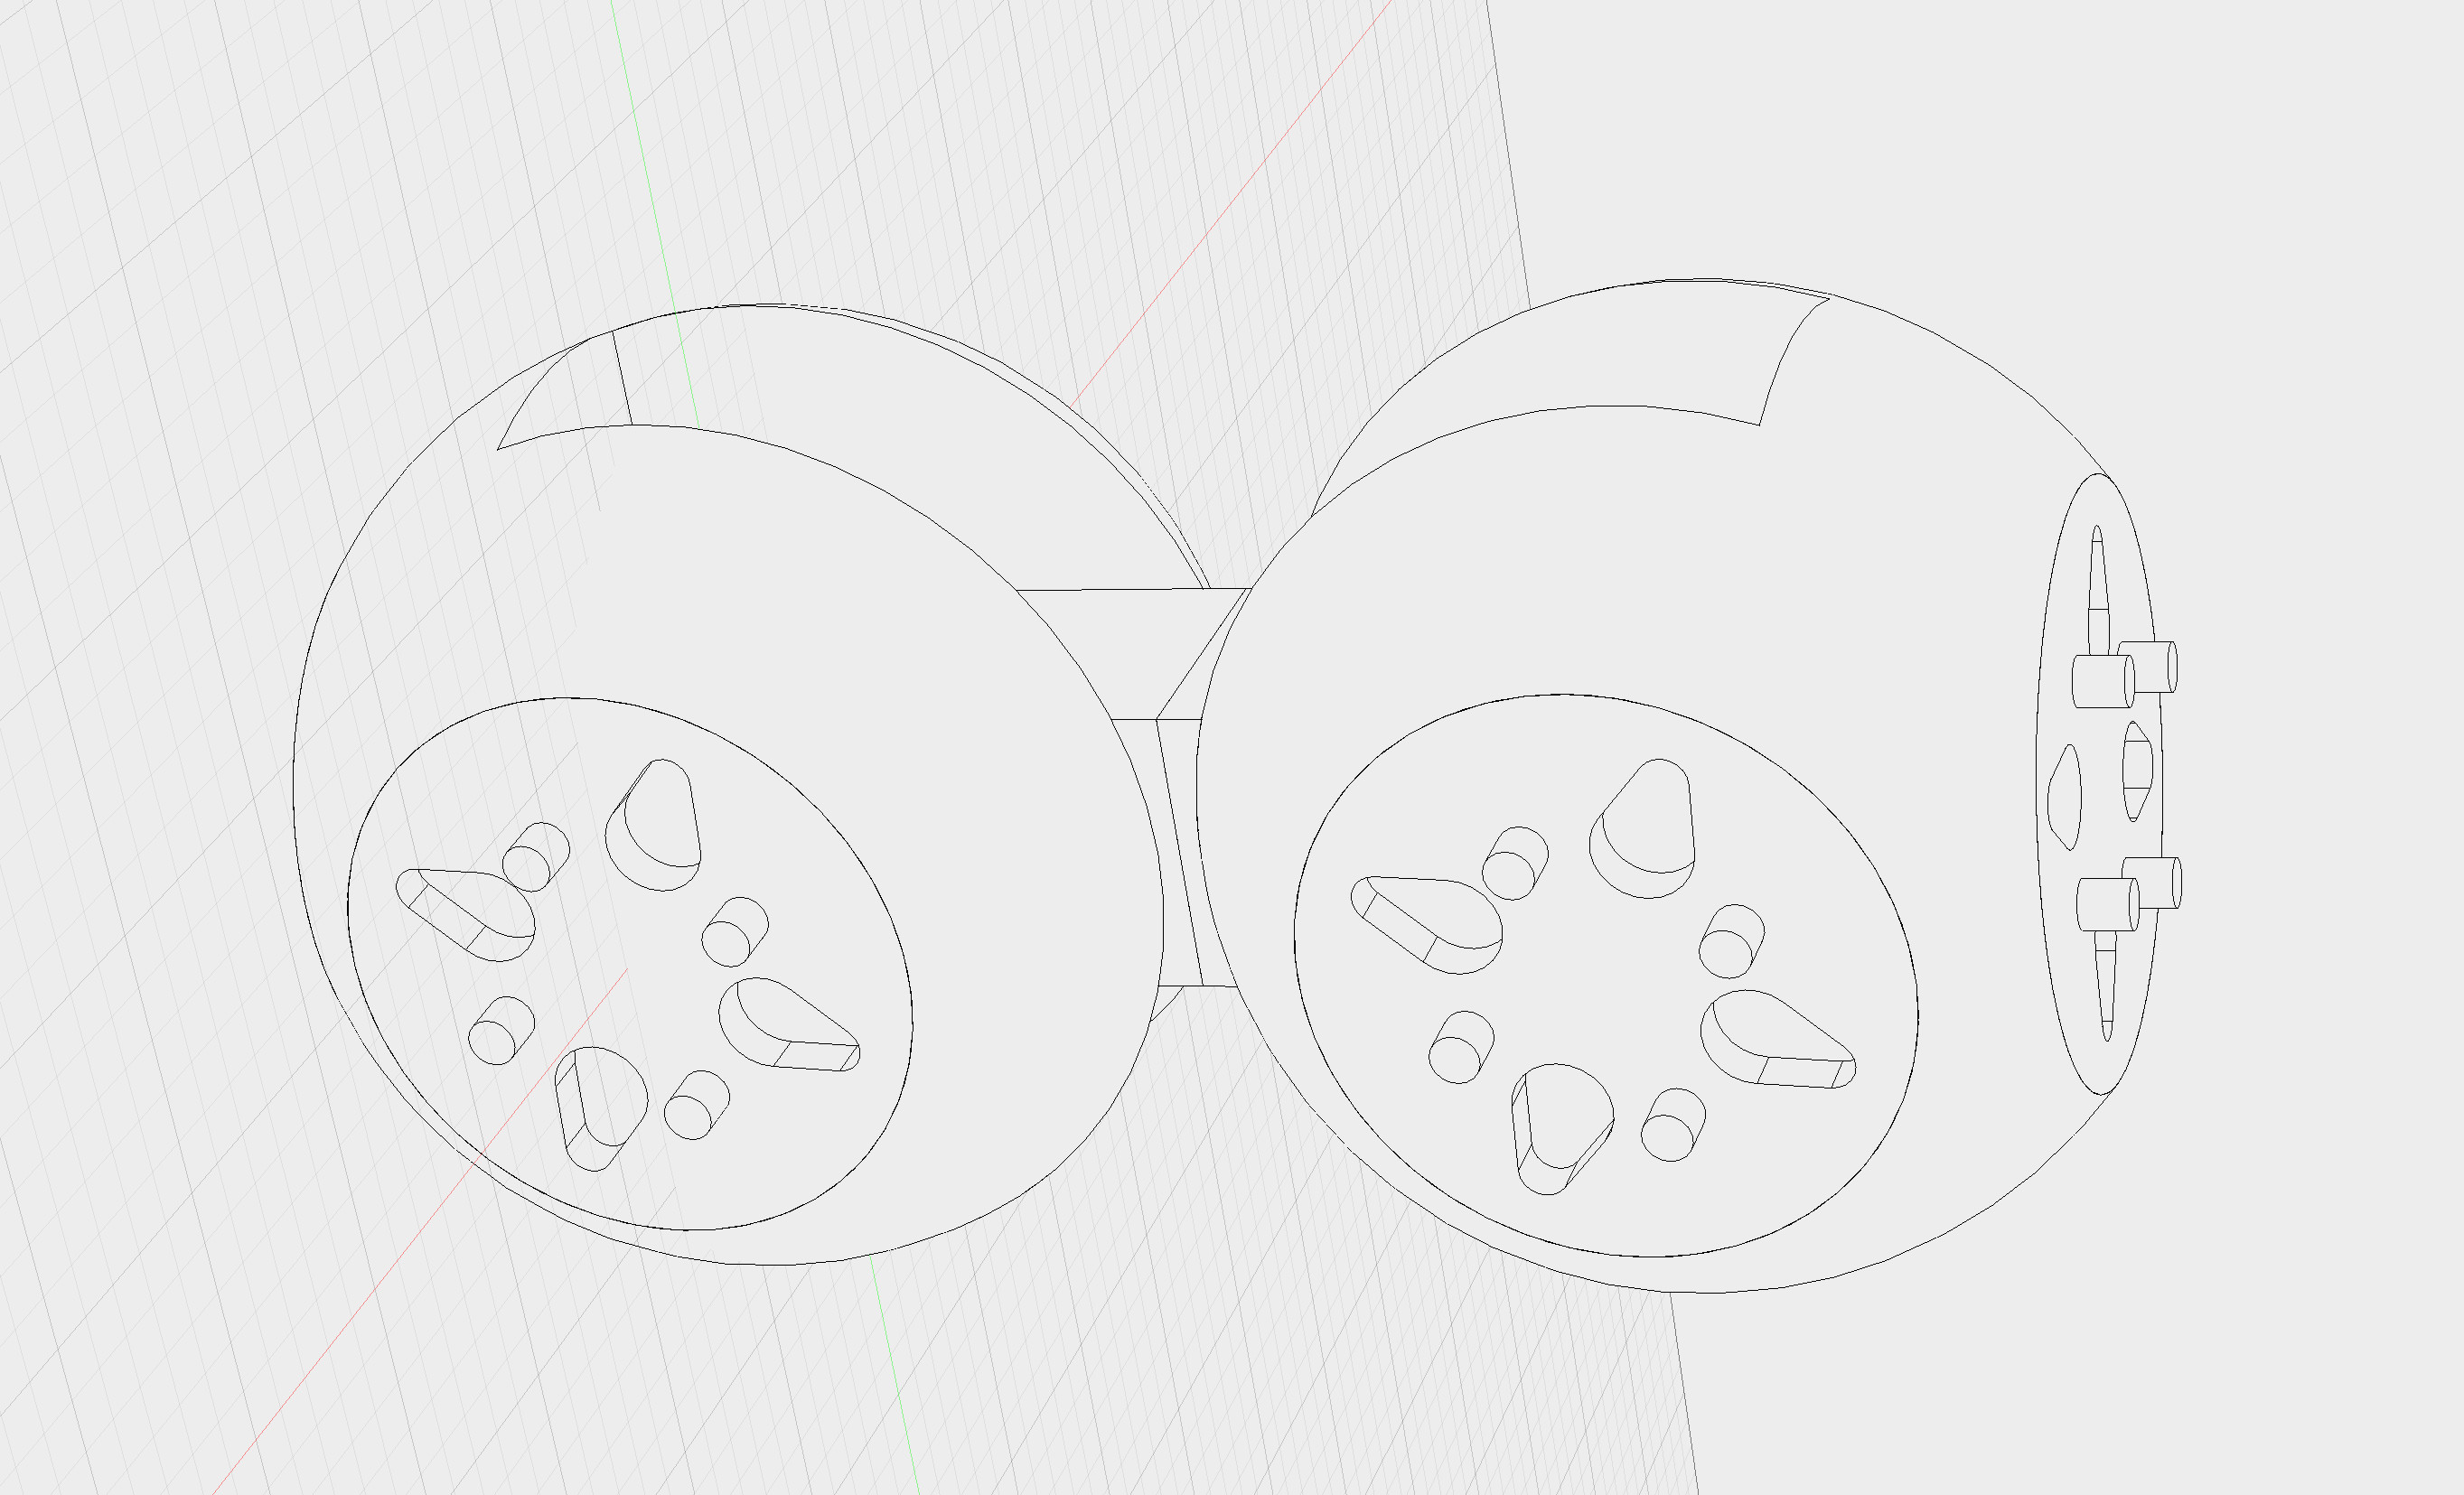
\includegraphics[width=\textwidth]{img/rofi1}
\end{frame}

\begin{frame}{Jak unikátní jsme?}
    \centering
    \only<2>{
        \begin{block}{MTRANS}
            \begin{figure}
                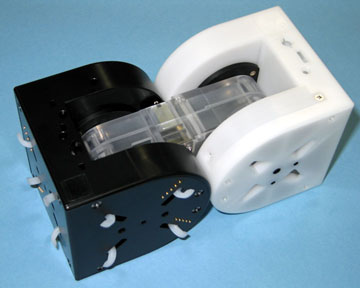
\includegraphics[width=0.8\textwidth]{img/mtran1}
            \end{figure}
        \end{block}
    }

    \only<3>{
        \begin{block}{SMORES}
            \begin{figure}
                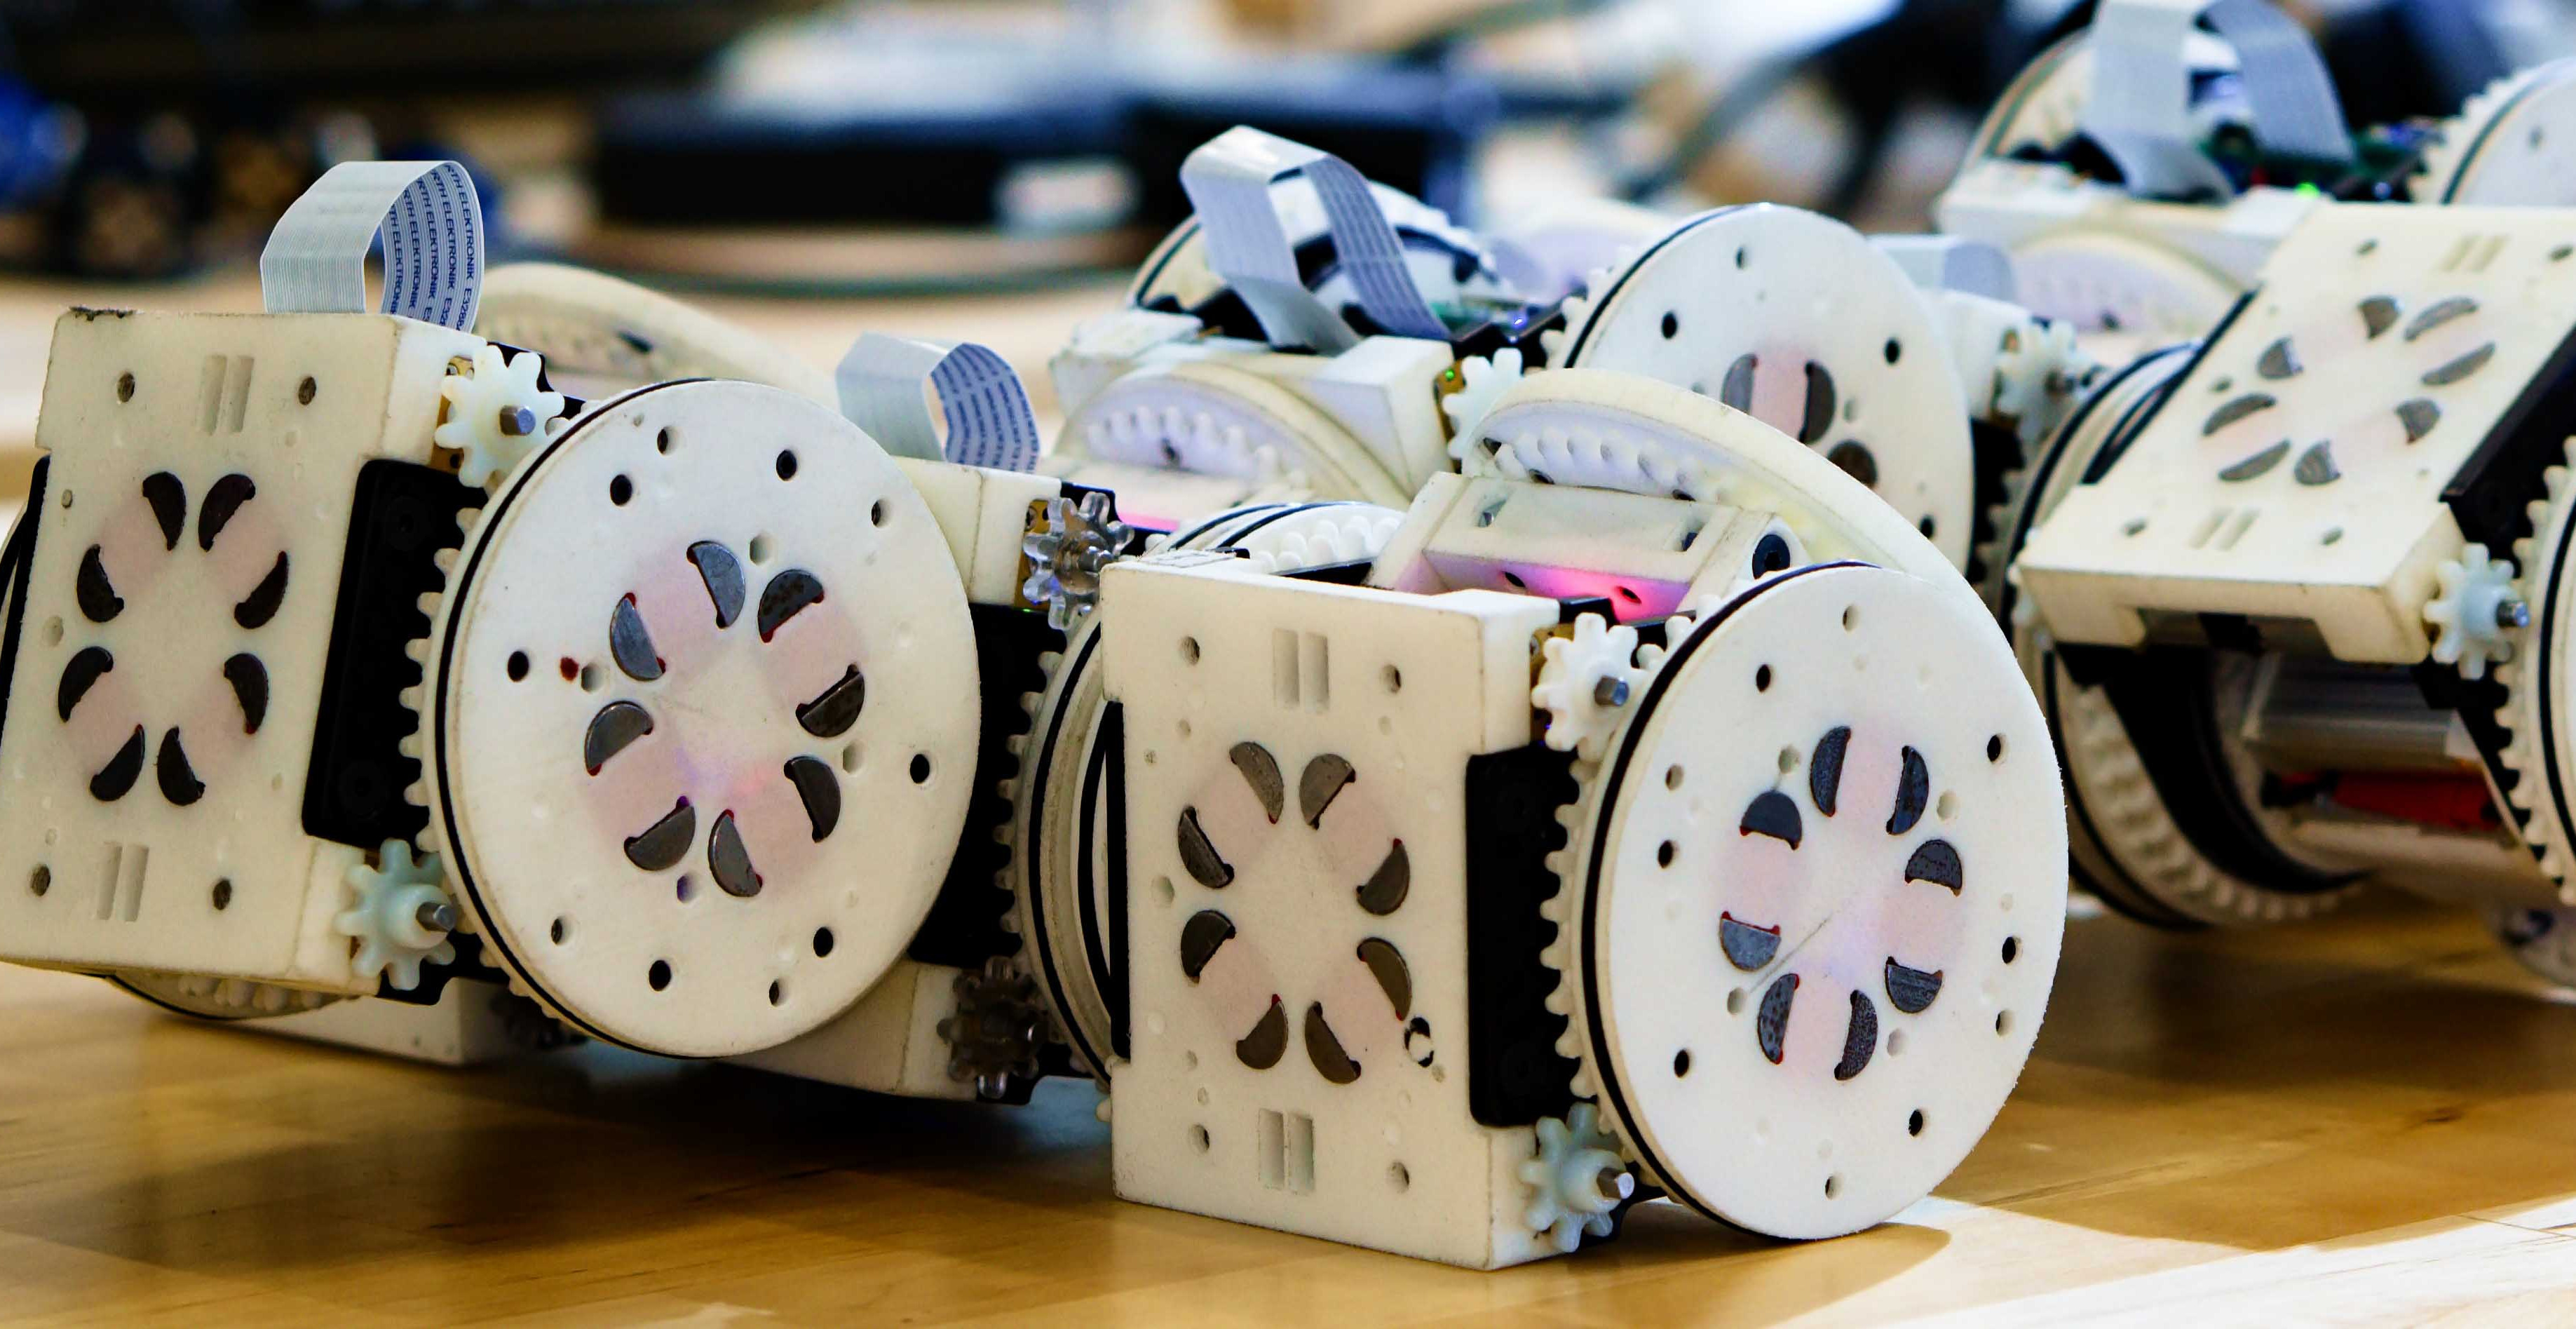
\includegraphics[width=0.8\textwidth]{img/smores1}
            \end{figure}
        \end{block}
    }

    \only<4>{
        \begin{block}{Roombots}
            \begin{figure}
                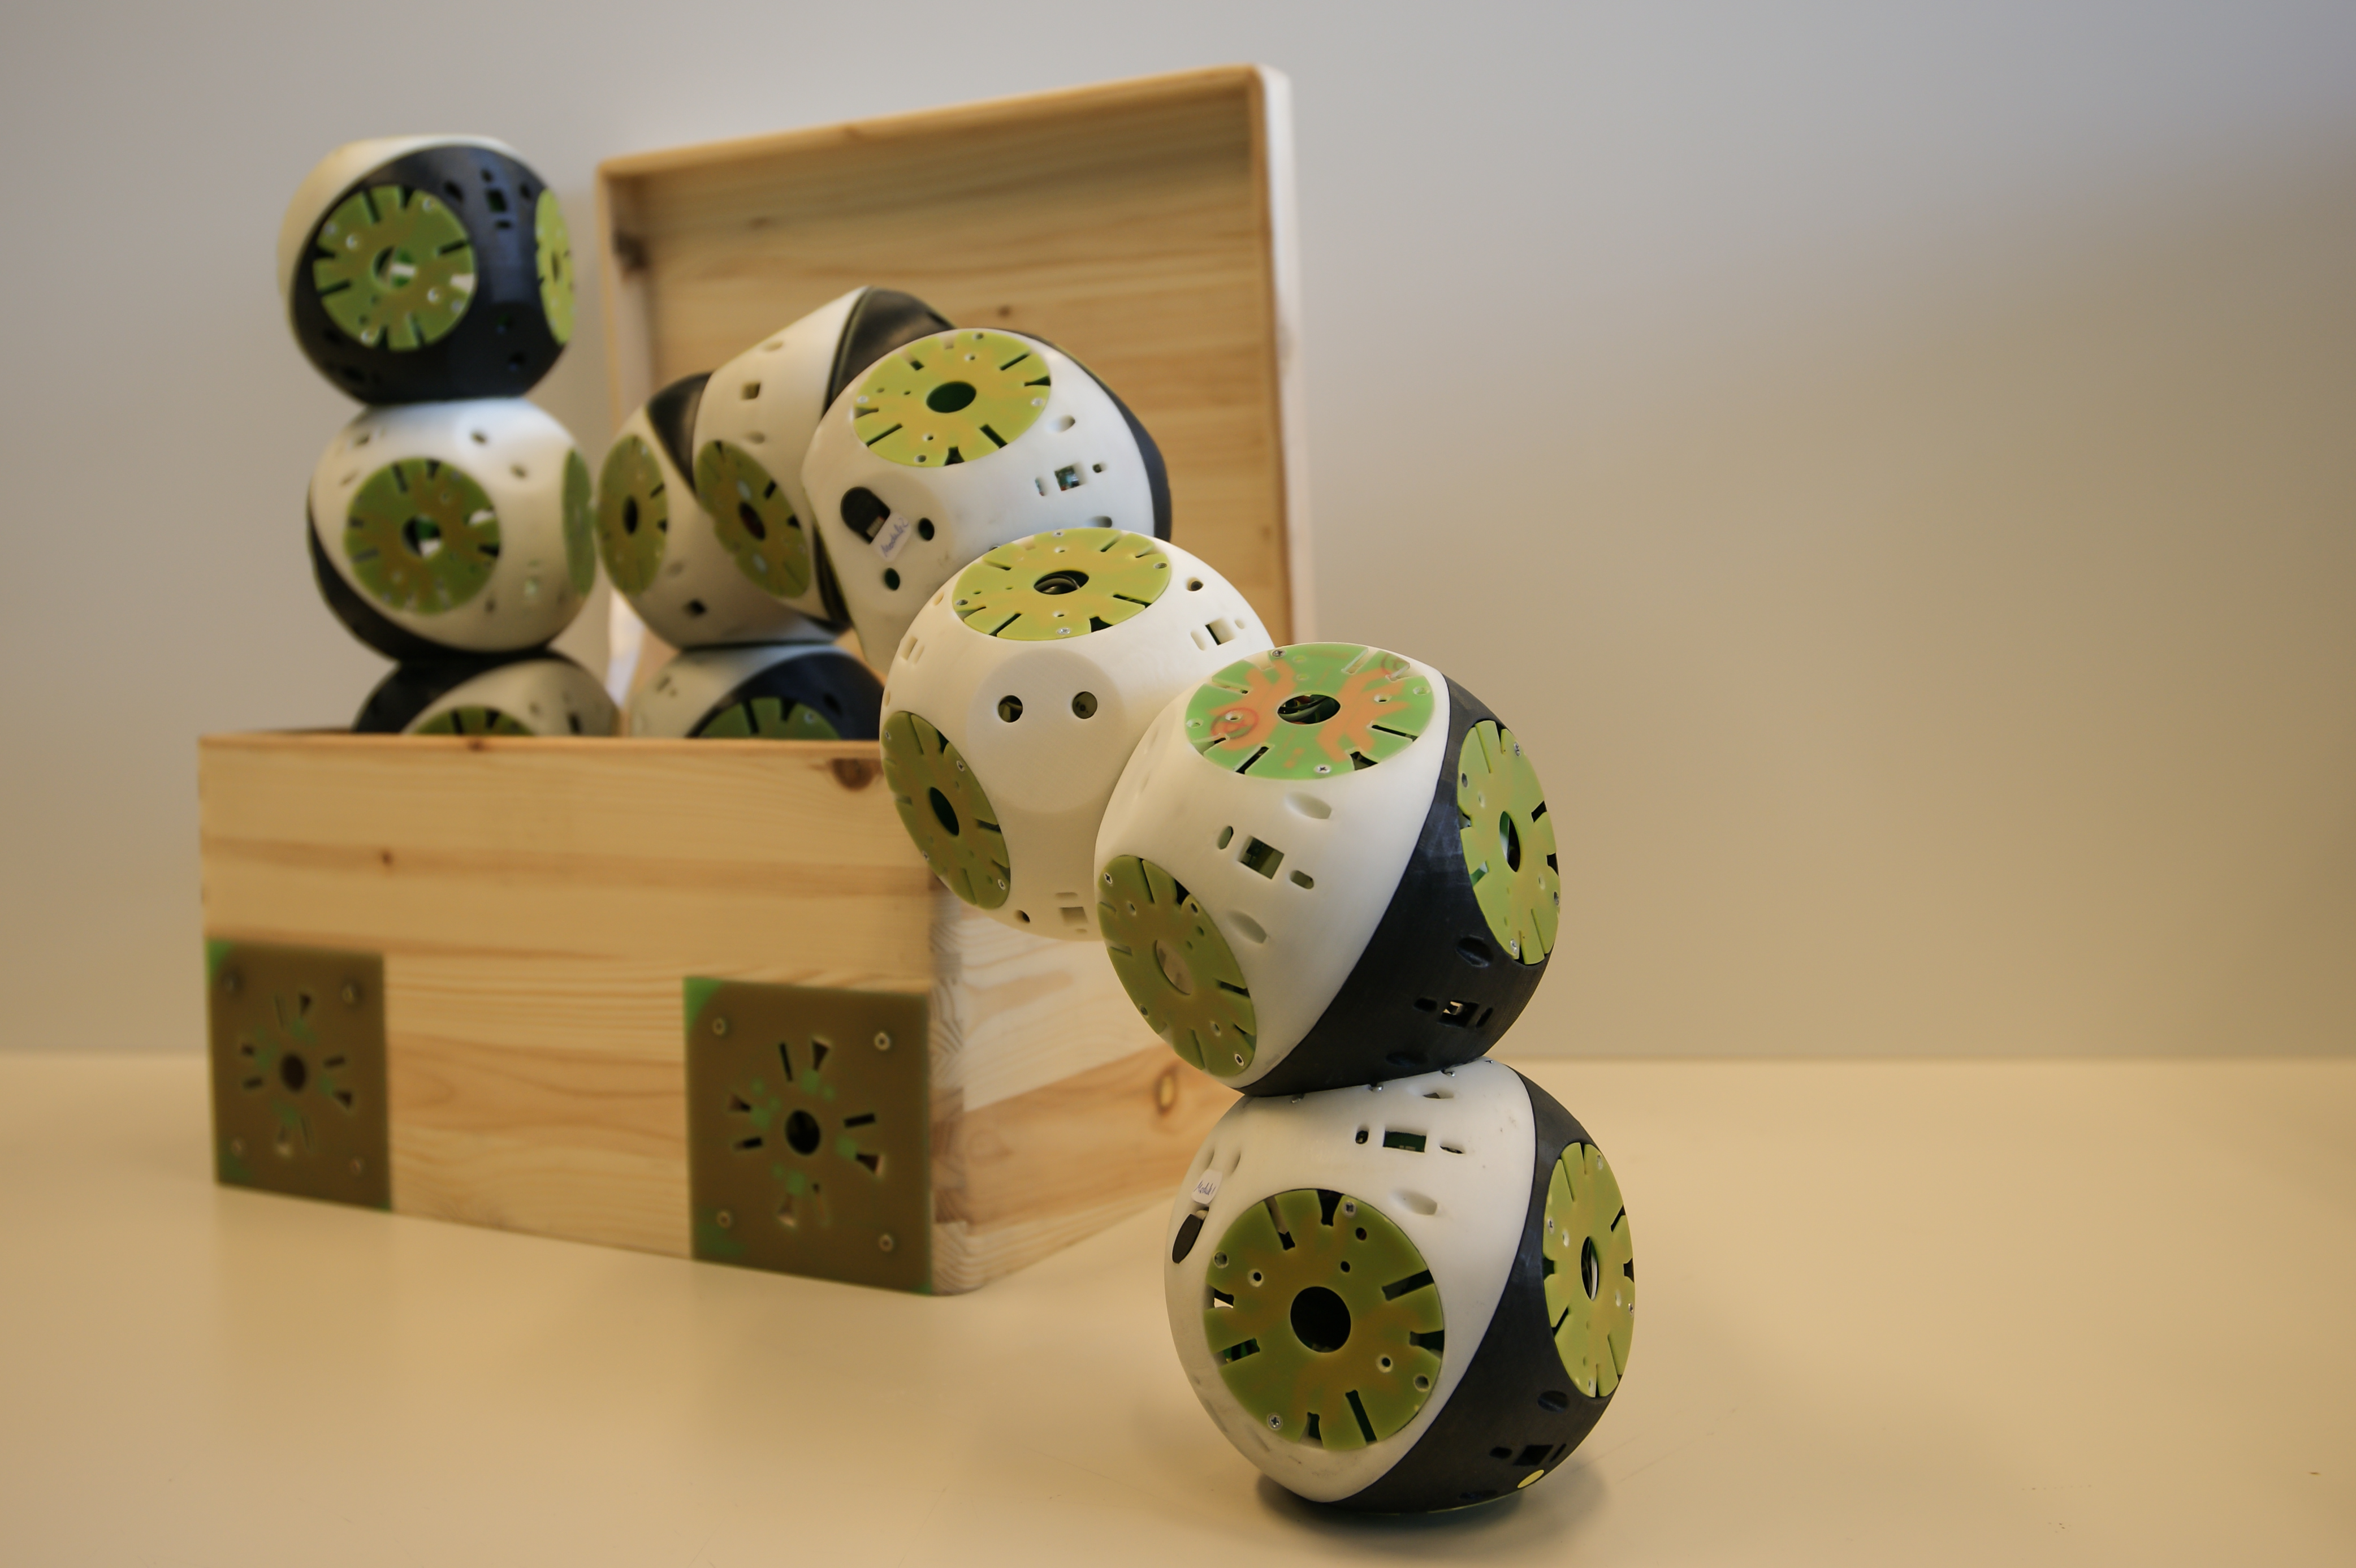
\includegraphics[width=0.8\textwidth]{img/roombot1}
            \end{figure}
        \end{block}
    }

\end{frame}

\begin{frame}{V čem jsme jiní?}
    \begin{itemize}
        \item čistá teorie vs. aplikace na skutečném HW
        \item symetričnost zamykání
        \item únosnost zamykání
        \item sdílený power managment
        \item grid-awareness

        \pause

        \item nemáme v plánu to zabalit
    \end{itemize}
\end{frame}

\begin{frame}{Vize projektu}
\end{frame}

\begin{frame}{Aktuální postup}
\end{frame}

\end{document}
